


in this section, we evaluate the context-aware encoding algorithm
and live streaming protocol. 


\begin{figure*}[ht]
  \centering
  \begin{subfigure}[t]{0.25\textwidth}
    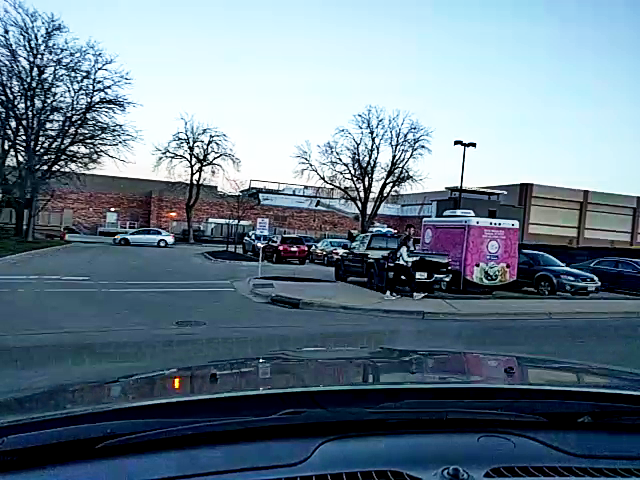
\includegraphics[width=\linewidth]{Figs/RTDrive/evaluation/frames/default_0.png}
  \end{subfigure}%
  \begin{subfigure}[t]{0.25\textwidth}
    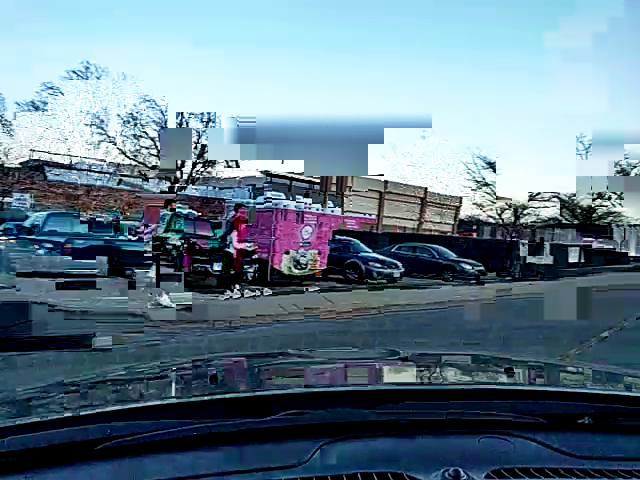
\includegraphics[width=\linewidth]{Figs/RTDrive/evaluation/frames/default_1.png}
  \end{subfigure}%
  \begin{subfigure}[t]{0.25\textwidth}
    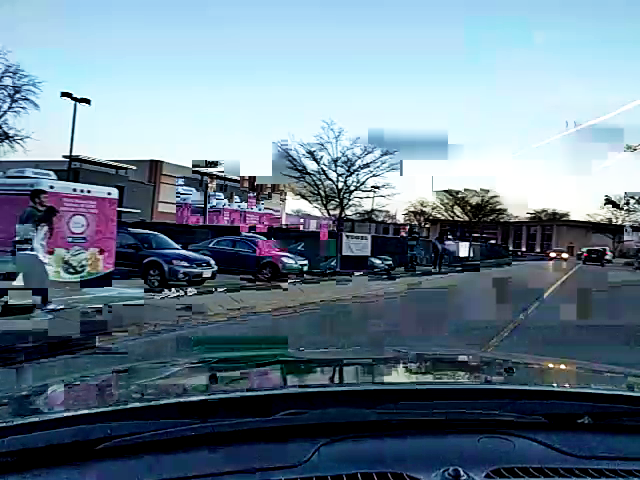
\includegraphics[width=\linewidth]{Figs/RTDrive/evaluation/frames/default_2.png}
  \end{subfigure}%
  \begin{subfigure}[t]{0.25\textwidth}
    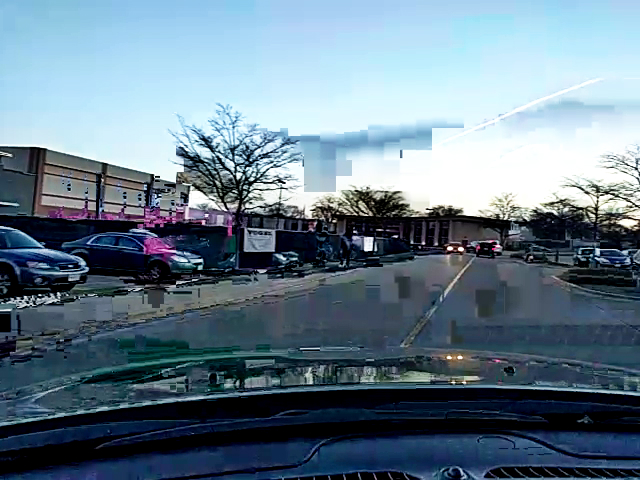
\includegraphics[width=\linewidth]{Figs/RTDrive/evaluation/frames/default_3.png}
  \end{subfigure}%
%  \begin{subfigure}[t]{0.2\textwidth}
%    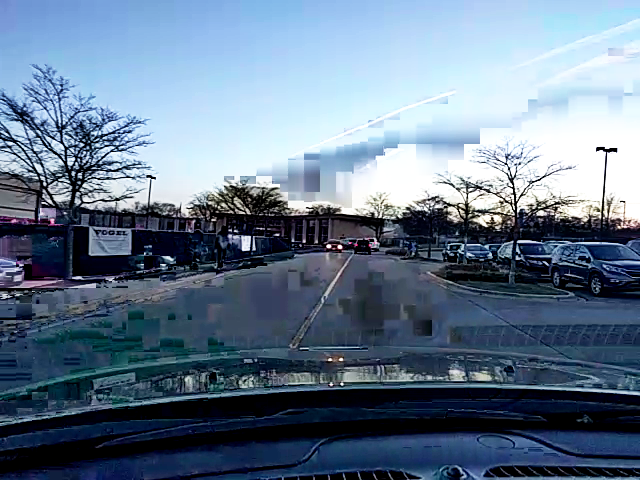
\includegraphics[width=\linewidth]{Figs/RTDrive/evaluation/frames/default_4.png}
%  \end{subfigure}%
  \label{default_encoding_images}
  
   \begin{subfigure}[t]{0.25\textwidth}
    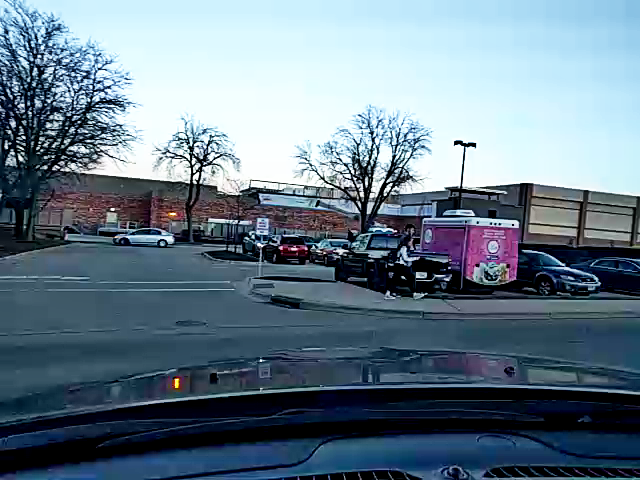
\includegraphics[width=\linewidth]{Figs/RTDrive/evaluation/frames/context_0.png}
  \end{subfigure}%
  \begin{subfigure}[t]{0.25\textwidth}
    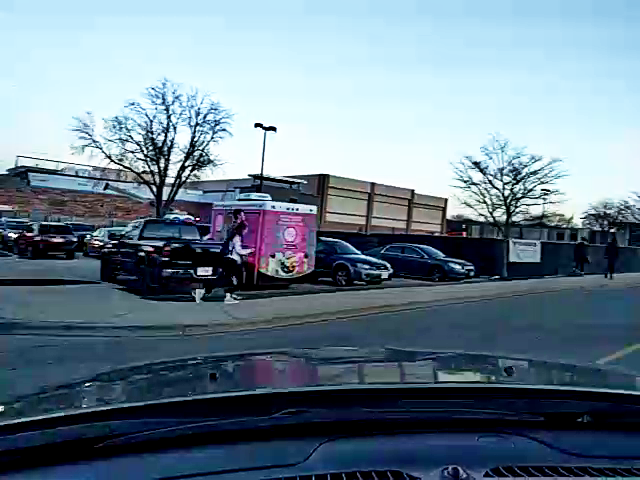
\includegraphics[width=\linewidth]{Figs/RTDrive/evaluation/frames/context_1.png}
  \end{subfigure}%
  \begin{subfigure}[t]{0.25\textwidth}
    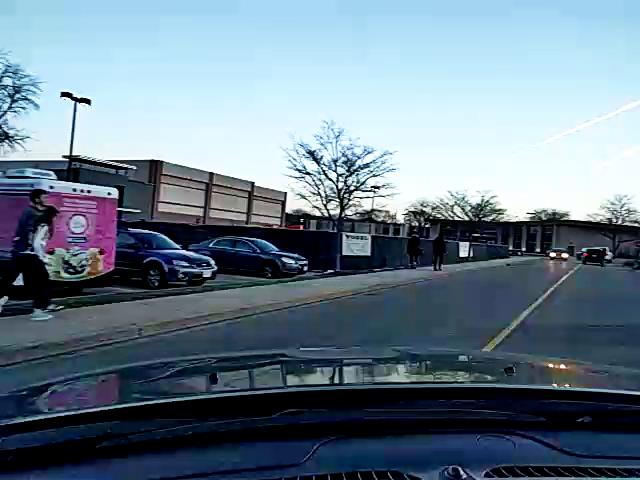
\includegraphics[width=\linewidth]{Figs/RTDrive/evaluation/frames/context_2.png}
  \end{subfigure}%
  \begin{subfigure}[t]{0.25\textwidth}
    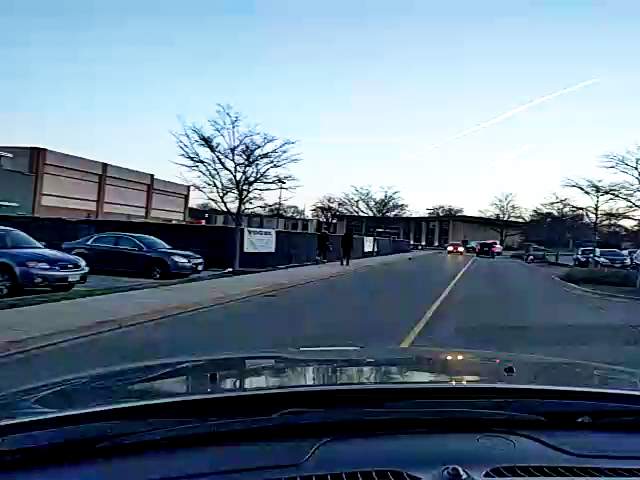
\includegraphics[width=\linewidth]{Figs/RTDrive/evaluation/frames/context_3.png}
  \end{subfigure}%
%  \begin{subfigure}[t]{0.2\textwidth}
%    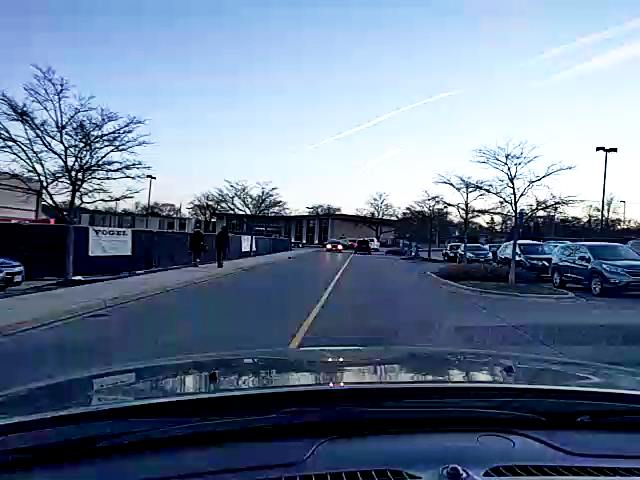
\includegraphics[width=\linewidth]{Figs/RTDrive/evaluation/frames/context_4.png}
%  \end{subfigure}%
  \caption{Images encoded by using fixed I-frame interval (above) and 
          context-aware encoding method (below) with 1mbps.
         The first frame is less clear than the default method, but the overall
         video quality is much higher. }
  \label{context_encoding_images}
\end{figure*}


\subsection{Context-Aware Video Encoding}

We compare the video quality of context-aware video encoding method 
with that of default encoding method in this section. 
We collect the raw frames under 5 different driving activities
of around 10 miles. 
The driving speed is from 0mph to 40mph and there are totally 22 
turns (exceed 60 degrees). 
At data collection time, we mount the Android phone in a vehicle
and drive the vehicle in different road segments, 
each raw frame is stored in the sdcard with predefined format. 
The raw frame data is collected through Android's \emph{onPreviewFrame}
callback function, where each captured frame is passed in 
as a byte array. 
Each raw frame starts with a fixed length header, which stores
the time and the real time sensor data. 
Each raw frame has the same size given the same resolution (640x480)
and raw frame format (Android YUV format) in a single trip. 
At evaluation time, we use Android to load in the raw frames
and encode the raw frames with different video encoding methods. 
The encoded frames are sent to the server to convert back
to the video, which is used to calculate the image quality. 


\subsubsection{Micro-benchmark}
\label{mico_context}

When load the raw frames, we encode them with context-aware video encoding
and the default H.264 video encoding, respectively. 
We use video encoding efficiency as a metric to evaluate video
encoding methods. 
We refer video encoding efficiency to video quality given the
same video encoding bitrate or the video encoding bitrate that
achieves the same video quality. 
We extract the frames when the car is marking a turn.
We replay the video by using 
the default encoding method with fixed
I-frame interval of 3s
and context-aware encoding method, 
and the sample images are shown in Fig. \ref{context_encoding_images}.
For the images with fixed I-frame
interval (above), 
all the images are blurred and distorted except for the first image (I-frame). 
For the images with context-aware encoding method (below),
all the images are with good quality.  

\subsubsection{Parameter Selection}
\label{sec_selection}


\begin{figure}[ht]
\centering
  \begin{subfigure}[t]{0.24\textwidth}
    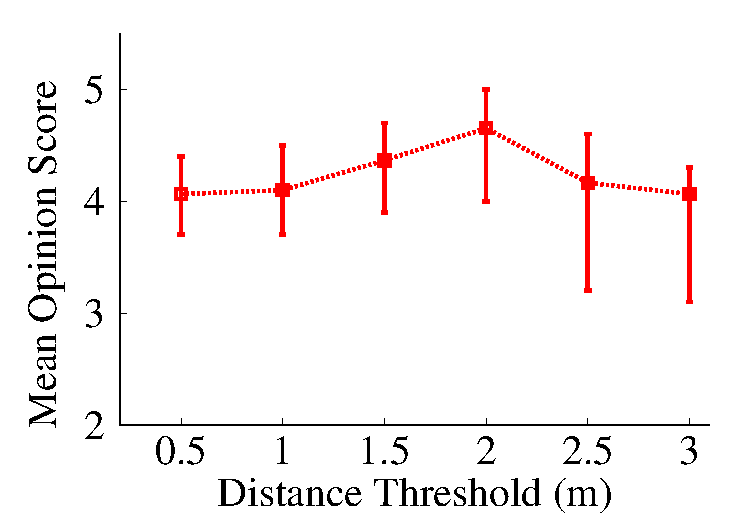
\includegraphics[width=\linewidth]{Figs/RTDrive/evaluation/context_dist.pdf}
    \vspace{-0.5cm}
    \caption{Distance threshold.}
    \label{param_dist}
  \end{subfigure}%
  \begin{subfigure}[t]{0.24\textwidth}
    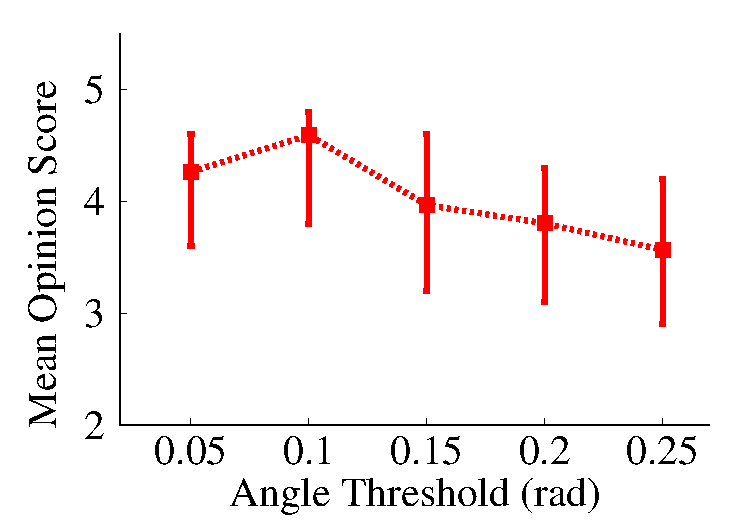
\includegraphics[width=\linewidth]{Figs/RTDrive/evaluation/context_gyro.pdf}
    \vspace{-0.5cm}
    \caption{Angle threshold.}
    \label{param_angle}
  \end{subfigure}%
  \vspace{-0.2cm}
  \caption{Sensitivity to parameters. }
  \label{parameters}
  \vspace{-0.25cm}
\centering
\end{figure}


The performance context-aware video encoding method depends on
two parameters, the distance and angular velocity thresholds.
The threshold is used to control how frequent the video 
encoder produces a I-frame. 
A lower threshold produces more I-frames and a higher
threshold produces more P-frames. 
To select the threshold parameters, we repeat the 
experiments in section \ref{mico_context} with different 
threshold settings.
We divided the trips into straight road and turns, 
and test different distance threshold on straight roads and
different angular velocity threshold in turns. 
The results are shown in Fig. \ref{parameters}. 
A high distance/angle threshold means there will be less 
I-frames (or a larger I-frame interval) and the frame quality heavily depends 
on the qualities of previous frames. 
As discussed in section \ref{sec_frame_encoding}, 
a large I-frame interval may cause bad quality P-frames 
when the scene changes frequently, 
which causes poor tail quality when using higher
thresholds. 

\subsubsection{Overall Performance}



\begin{figure}[t]
\centering
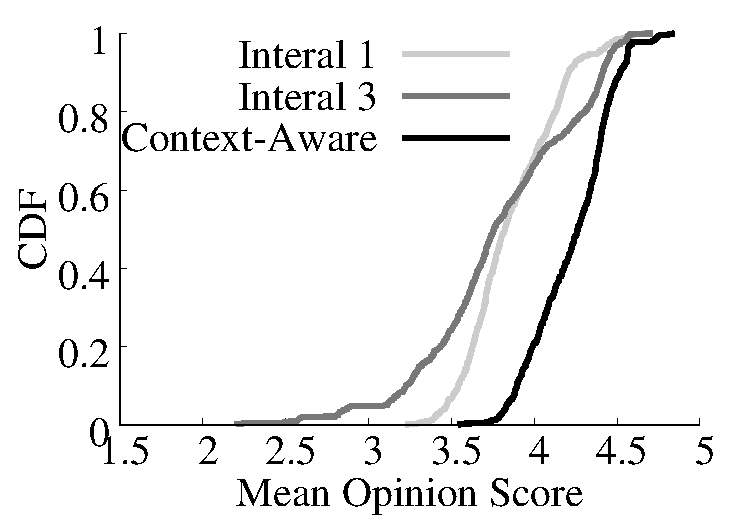
\includegraphics[width=2.8in,angle=0]{Figs/RTDrive/evaluation/context_quality.pdf}
\caption{Video quality under default encoding method
and context-aware encoding method.}
\vspace{-0.2cm}
\label{context_quality}
\centering
\end{figure}


The overall performance of context-aware video encoding method is evaluated
through all the 5 trips we collected. 
We use the parameter settings selected in section \ref{sec_selection}.
The default comparison method uses a fixed I-frame interval of 1s and 3s.
As shown in Fig. \ref{context_quality}, 
if we use a small I-frame interval (1s in this case), the deviation of the image
qualities are small while the average qualities are dropped
as the frame differences are not fully utilized. 
If we use a larger I-frame interval (3s in this case), 
the deviation of the image qualities are larger while some I-frames
have better quality than the rest.
Context-aware encoding is able to select I-frame and P-frame
based on potential frame difference changes, 
which lead better overall performance than using
fixed interval encoding method.  

\subsection{Consistent-Latency Remote Control}


\begin{figure*}[ht]
  \begin{subfigure}[t]{0.20\textwidth}
    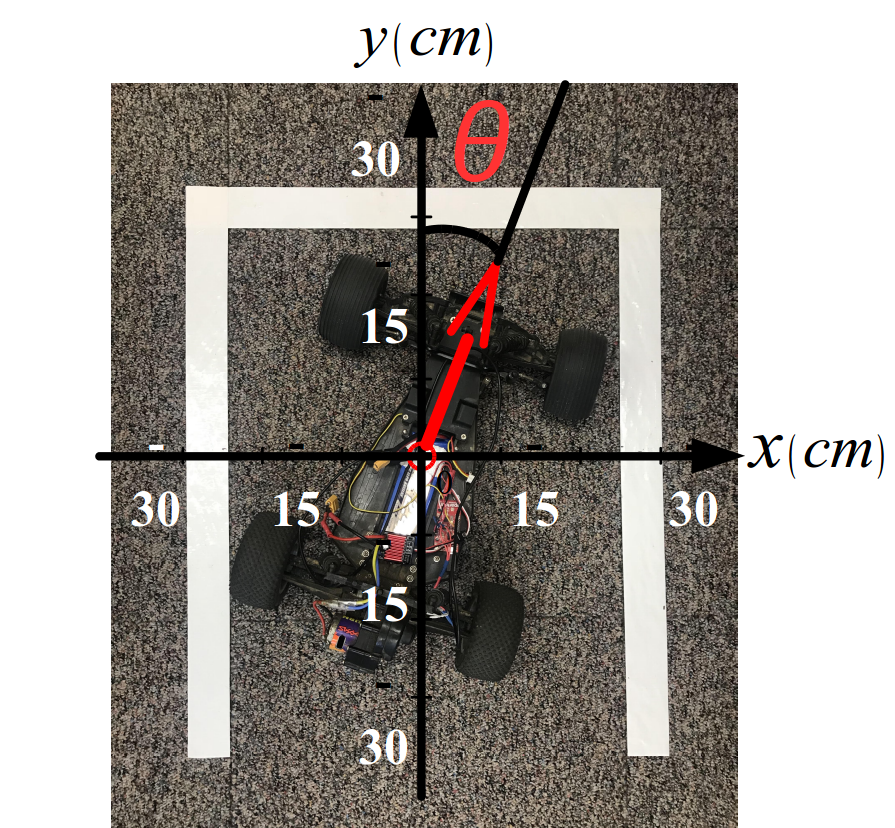
\includegraphics[width=\linewidth]{Figs/RTDrive/evaluation/car.png}
    \caption{Parking spot.}
    \label{parking_car}
  \end{subfigure}
  \begin{subfigure}[t]{0.26\textwidth}
    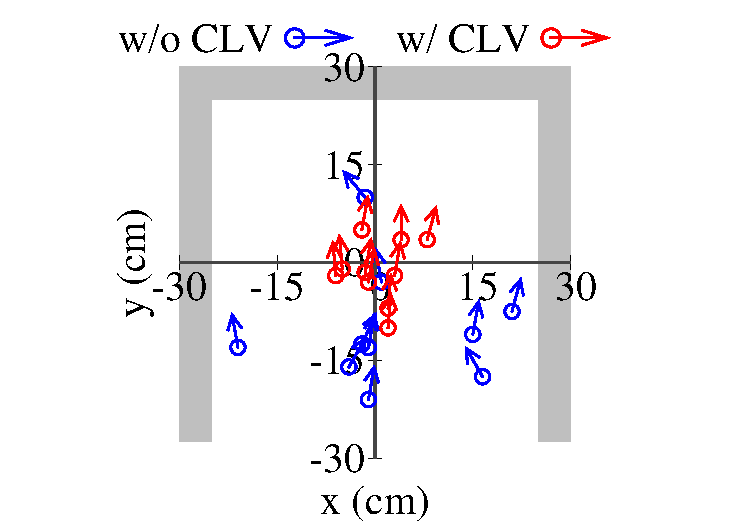
\includegraphics[width=\linewidth]{Figs/RTDrive/evaluation/position_fewerpoints.pdf}
    \caption{Parking control illustration.}
    \label{consistent:illustration}
  \end{subfigure}%
  \begin{subfigure}[t]{0.26\textwidth}
    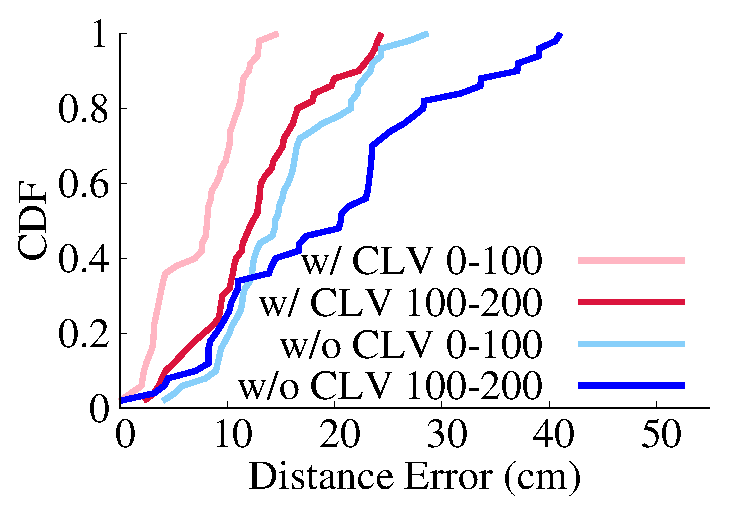
\includegraphics[width=\linewidth]{Figs/RTDrive/evaluation/Distance.pdf}
    \caption{Parking distance error.}
    \label{consistent:distance}
  \end{subfigure}%
  \begin{subfigure}[t]{0.26\textwidth}
    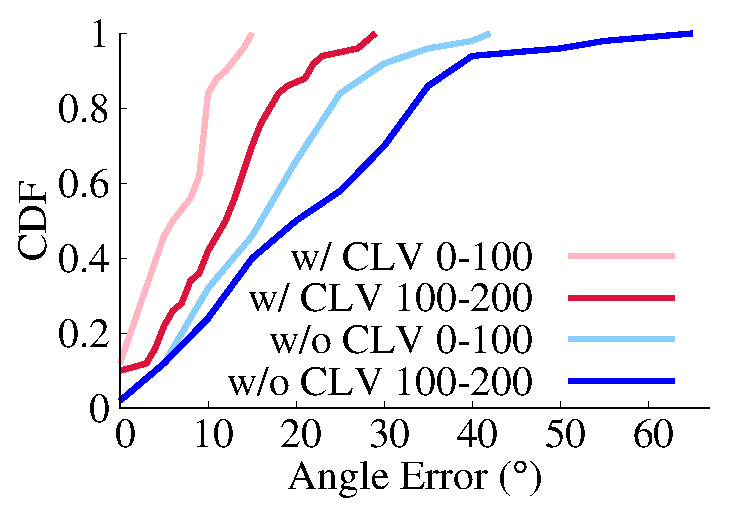
\includegraphics[width=\linewidth]{Figs/RTDrive/evaluation/Angle.pdf}
    \caption{Parking angle error.}
    \label{consistent:angle}
  \end{subfigure}%
  \caption{The precision of remote control of different operators under 
various latency settings.}
  \label{feasibility}
  \vspace{-0.2cm}
\end{figure*}


To understand the impact of consistent-latency on
steering and speed control of the vehicle, 
we conduct user study on a parking task.
Parking is one of most challenging driving activities, 
and a parking lot experiment can test the most fundamental 
controls of vehicle of the operators, steering and speed.
This experiment is conducted under indoor Wi-Fi environment. 
 
As shown in Fig. \ref{parking_car}, 
we draw a parking spot on the ground by using white tapes.
The remote control car is 5 meters vertical distance and 1 meter horizontal distance away. 
The operators are asked to drive the car by using
steering and forwarding control.
The backward control is disabled so that the operator has no
chance to do readjustment and the operator
has only one chance to park the car in the spot.   
The operators can only see the live streaming video on the server monitor. 
The whole setup is similar to a car racing game, except
the operator is controlling a real car. 


The participates start with 10 test drives to get familiar with 
the environment and get feedback themselves for their
control precision and parking performance. 
After the test drive, they are asked to drive the car under
different latency and parameter settings. 
The experiment consists of 20 groups with extra latency
of 0ms, 40ms, 80ms, 120ms, 160ms and 200ms. 
Half of the experiment groups are conducted with consistent-latency
enabled and half are not.
The experiment are randomly generated and the participants
do not know the settings at the time they control the vehicle. 


We use distance error and angle error to evaluate
parking performance. 
Distance error refers to the distance of the parked car to the distance
of the center of the parking spot. 
Angle error refers to te difference between the parked direction and vertical direction.
We divide the results into two latency groups, 0-100ms and 100-200ms. 
With CLV, the both the median distance error and median angle error
are reduced by half under different latency settings. 
The parking performance of one participate under 80ms latency is shown
in Fig. \ref{consistent:illustration}. 
In the cases there is no CLV, the video frames may be lagged or jumped due to
the variance of wireless network latency and bandwidth. 
With CLV, the participates have smoother view, so that 
the control can be more precise as they can 
``predict'' the impact of the latency. 



\subsection{Live Streaming Protocol}

We evaluate the live streaming protocol in this section. 
We compare the performance of UDP and TCP, with and without
FEC. 
We also present performance of bandwidth and loss rate
estimation module of the protocol. 

\subsubsection{FEC and Video Quality}

\begin{figure}[t]
\centering
\vspace{-0.3cm}
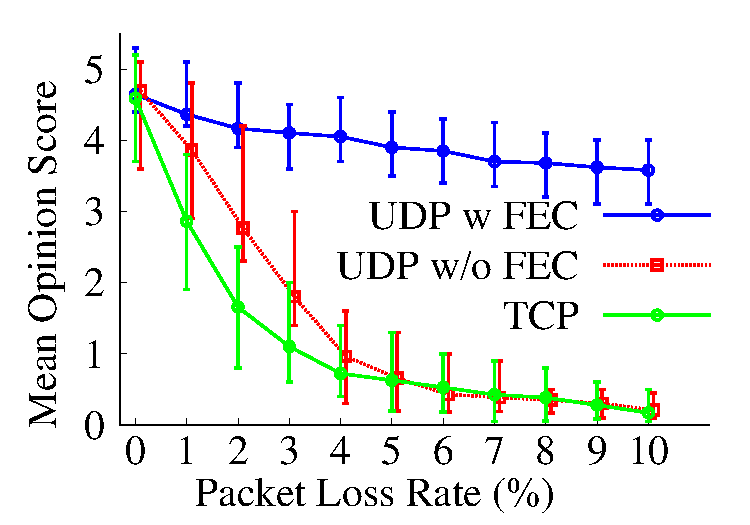
\includegraphics[width=2.6in,angle=0]{Figs/RTDrive/evaluation/video_quality_errorbars.pdf}
\vspace{-0.3cm}
\caption{Video quality under different loss rates.}
\vspace{-0.2cm}
\label{loss_quality}
\centering
\end{figure}


\begin{figure*}[ht]
\centering
  \begin{subfigure}[t]{0.33\textwidth}
    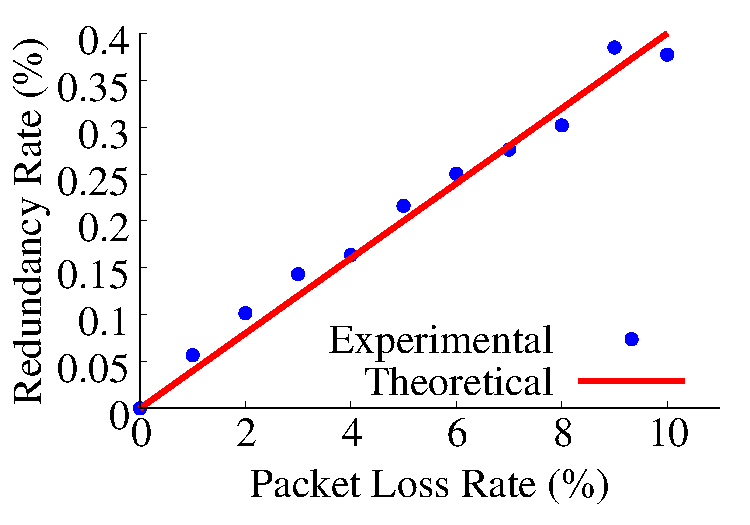
\includegraphics[width=\linewidth]{Figs/RTDrive/evaluation/fec_ratio.pdf}
    \vspace{-0.5cm}
    \caption{FEC ratio under various loss rate.}
    \label{fec_ratio}
  \end{subfigure}%
  \begin{subfigure}[t]{0.33\textwidth}
    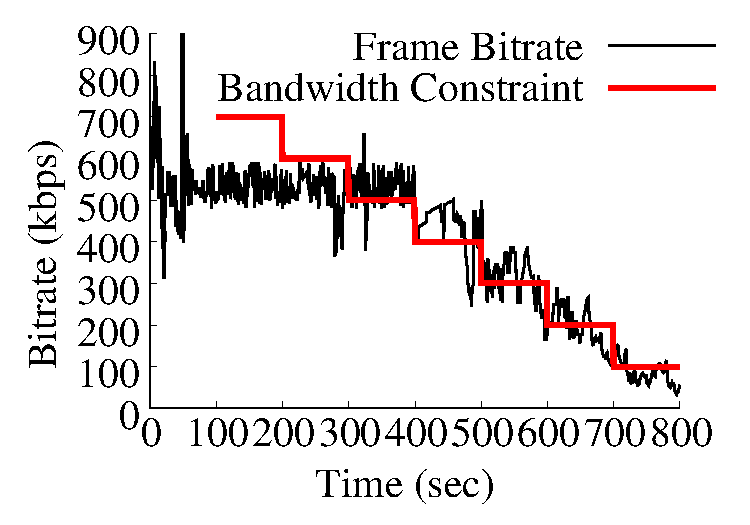
\includegraphics[width=\linewidth]{Figs/RTDrive/evaluation/bandwidth.pdf}
    \vspace{-0.5cm}
    \caption{Bandwidth estimation and adaptation.}
    \label{bandwidth}
  \end{subfigure}%
  \begin{subfigure}[t]{0.33\textwidth}
    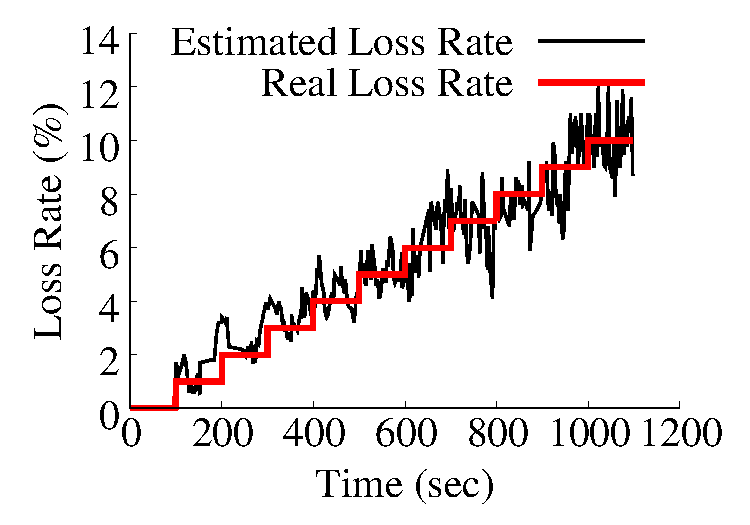
\includegraphics[width=\linewidth]{Figs/RTDrive/evaluation/lossrate.pdf}
    \vspace{-0.5cm}
    \caption{Loss rate estimation.}
    \label{loss_rate}
  \end{subfigure}%
  \vspace{-0.3cm}
  \caption{Estimation accuracy of transmission protocols. }
  \label{feasibility}
  \vspace{-0.2cm}
\centering
\end{figure*}



We evaluate the impact of packet loss rate on video quality, 
with and without FEC, respectively. 
We use the Android app to record and stream a driving video 
we recorded for trace replay experiments. 
The server connects with the router through a Ethernet 
cable and the Android connects with the same router
through Wi-Fi.  
The server will store the streaming video locally
and then use the video quality check tool 
to calculate the quality. 
The results are shown in Fig. \ref{loss_quality}. 
If there is no FEC or similar redundancy mechanism, 
a loss rate of 3\% makes most frames distorted and hard to view. 
Video encoding algorithm is sensitive to packet loss. 
If one fraction of a I-frame get lost, that fraction
cannot be displayed properly. 
Also, the quality of the following P-frame will be even worse 
since the compression relies on the missing fraction 
and the video decoder cannot recover properly. 
The future P-frame which relies on previous I-frame
and P-frame will have even worse quality for
the same reason. 
The loss of one fraction will propagate to all of the 
following P-frames.  
With FEC encoding, the server side can recover most of the 
frames. 


\subsubsection{UDP and TCP}


We perform a comparative benchmark of UDP and TCP under various 
loss rate, and the results are shown in Fig. \ref{loss_quality}. 
Other modules are using the default settings. 
In UDP measurement, the FEC is enabled for fair
comparison. 
In TCP measurement, the FEC is disabled since
TCP is lossless protocol. 
Unlike TCP, the latency of UDP is insensitive to packet loss. 
As shown in Fig. \ref{loss_quality}, the latency of UDP is not sensitive
to packet loss as the transmission rate is smaller
than available bandwidth. 
TCP is sensitive to packet loss, as TCP will treat packet loss
as congestion and then try to slow down transmission by 
The higher latency of TCP at higher loss rate is caused by 
two reasons. 
First, if one frame packet is lost, then the whole frame has to
wait for the retransmission of that packet, 
which cause an extra RTT. 
Second, the TCP congestion control will slow down future transmission
upon packet loss, which increase the buffering time of 
future frames. 
Under loss rate of more than 2\%, the streaming video will freeze
frequently and cause the video not able to view. 



\subsubsection{Bandwidth and Packet Loss Rate Estimation}

To evaluate how our live streaming protocol performs under 
different wireless network conditions, 
we emulate various loss and latency under indoor Wi-Fi
environments.  
We use netem and Intermediate Functional Block pseudo-device \cite{netem} to 
create loss, extra network delay and bandwidth constraints. 
In this experiment, we add constraints on the bandwidth of the 
Ethernet port of the server. 
The server connects with the router with an Ethernet cable. 
The Android connects with the router through Wi-Fi. 
We decrease the bandwidth constraints from $700kbps$ to $100kbps$. 
The Android streams the video to the server and adapt 
the video bitrate according to the estimation and adaptation algorithm
described in section \label{sec_bandwidth}. 
Similar to bandwidth constraint, we set packet loss rate by using 
netem \cite{netem}. 
The loss rate estimation result is shown in Fig. \ref{loss_rate}. 
We increase the loss rate 1\% for every 100s, 
and our protocol can track packet loss rate closely. 


\subsubsection{End-to-End Latency Breakdown}


\begin{table*}[t]
  \centering
  \caption[latency]{Latency Breakdown}
  \vspace{-0.0cm}
  \label{latency}
  \begin{tabular}{|c|c|c|c|c|c|c|}
  \hline
Modules & Lane Detector & Object Detector  &  Frame Encoding  &  Serial & Wireless Network  & End-to-end  
\\  \hline
Latency & 38ms & 30ms & 21-42ms & 2-10ms & 40-200ms & 200-500ms
\\  \hline      
  \end{tabular}
  \vspace{-0.0cm}
\end{table*}


\begin{figure}[t]
\centering
\vspace{-0.0cm}
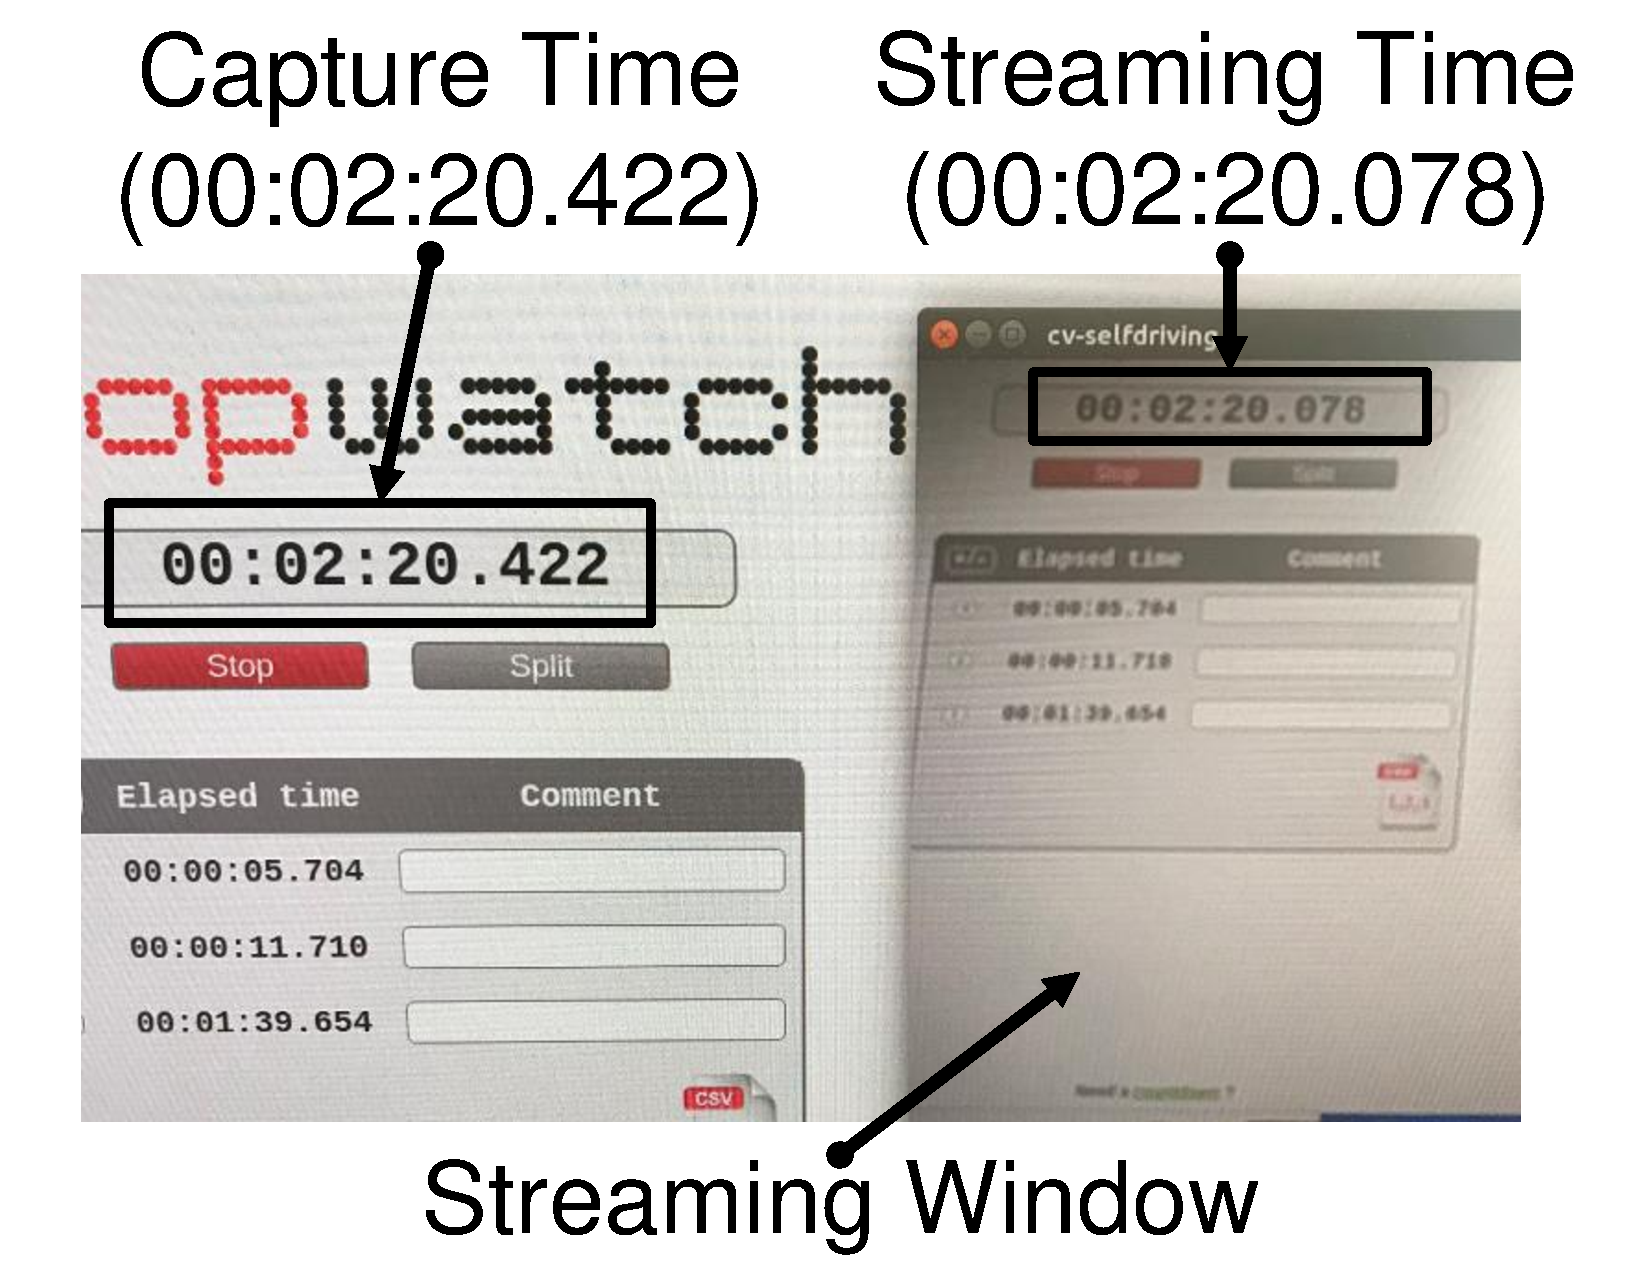
\includegraphics[width=2.4in,angle=0]{Figs/RTDrive/evaluation/endtoend.pdf}
\vspace{-0.2cm}
\caption{The end-to-end streaming and display latency measurement.}
\vspace{-0.2cm}
\label{endtoend}
\centering
\end{figure}


We benchmark the latency of each module and summarize the 
results in Table \ref{latency}. 
The latency of lane detector, frame encoding and FEC are measured
in the Android app. 
Each module is called through a API function. 
A timer recorded the timestamp both before and after calling this function and 
the difference is the latency caused by this module. 
It should be noted that object identification can be separated 
into another thread to reduce the streaming latency, 
and we left such optimization and the evaluation into future work.  
The round-trip latency of serial communication between Android device and 
Arduino board is measured by message with timestamp.  
The round-trip latency is frame latency measured by packet timestamps. 
End-to-end latency is the latency between the time the frame is captured
and the time the frame is viewed by user through streaming. 
To measure the end-to-end latency, we start a millisecond timer
on the server, and use the Android device to stream the 
timer to the same screen. 
As shown in Fig. \ref{endtoend}, we take the screenshot of 
the streaming window as well as the timer.
The streaming window is the video display on the server for the
streaming videos from the Android device. 
The difference between the two timer is the end-to-end latency
for video streaming.  
We illustrate that it suffers 200-500ms end-to-end display latency 
when streaming 640x480 resolution frames by using
standard video compression algorithms \cite{marpe2006h}
under current LTE networks. 
Compared with average driver reaction time of 0.7-2.4 seconds \cite{taoka1989brake}, 
the extra delay is tolerable for human operator
to control the car remotely.  

To reduce the end-to-end streaming latency, there are several techniques 
can be used. 
A higher performance system board can be used to replace the Android phone. 
Some optimization techniques such as \cite{likamwa2015starfish} can be used
to avoid duplicate operations and reduce image processing latency. 
The video encoding speed can be improved by dedicated hardware and
the wireless communication speed can also be improved. 
In the Wi-Fi setting, the Android Wi-Fi module enters sleep state
every 100ms, even the highest performance is enabled. 
Such sleep state causes 50-100ms one-way latency. 
Also, 5G and/or better designed wireless communication infrastructure and protocol
can be used to reduce the communication latency. 



